\documentclass[1p]{elsarticle_modified}
%\bibliographystyle{elsarticle-num}

%\usepackage[colorlinks]{hyperref}
%\usepackage{abbrmath_seonhwa} %\Abb, \Ascr, \Acal ,\Abf, \Afrak
\usepackage{amsfonts}
\usepackage{amssymb}
\usepackage{amsmath}
\usepackage{amsthm}
\usepackage{scalefnt}
\usepackage{amsbsy}
\usepackage{kotex}
\usepackage{caption}
\usepackage{subfig}
\usepackage{color}
\usepackage{graphicx}
\usepackage{xcolor} %% white, black, red, green, blue, cyan, magenta, yellow
\usepackage{float}
\usepackage{setspace}
\usepackage{hyperref}

\usepackage{tikz}
\usetikzlibrary{arrows}

\usepackage{multirow}
\usepackage{array} % fixed length table
\usepackage{hhline}

%%%%%%%%%%%%%%%%%%%%%
\makeatletter
\renewcommand*\env@matrix[1][\arraystretch]{%
	\edef\arraystretch{#1}%
	\hskip -\arraycolsep
	\let\@ifnextchar\new@ifnextchar
	\array{*\c@MaxMatrixCols c}}
\makeatother %https://tex.stackexchange.com/questions/14071/how-can-i-increase-the-line-spacing-in-a-matrix
%%%%%%%%%%%%%%%

\usepackage[normalem]{ulem}

\newcommand{\msout}[1]{\ifmmode\text{\sout{\ensuremath{#1}}}\else\sout{#1}\fi}
%SOURCE: \msout is \stkout macro in https://tex.stackexchange.com/questions/20609/strikeout-in-math-mode

\newcommand{\cancel}[1]{
	\ifmmode
	{\color{red}\msout{#1}}
	\else
	{\color{red}\sout{#1}}
	\fi
}

\newcommand{\add}[1]{
	{\color{blue}\uwave{#1}}
}

\newcommand{\replace}[2]{
	\ifmmode
	{\color{red}\msout{#1}}{\color{blue}\uwave{#2}}
	\else
	{\color{red}\sout{#1}}{\color{blue}\uwave{#2}}
	\fi
}

\newcommand{\Sol}{\mathcal{S}} %segment
\newcommand{\D}{D} %diagram
\newcommand{\A}{\mathcal{A}} %arc


%%%%%%%%%%%%%%%%%%%%%%%%%%%%%5 test

\def\sl{\operatorname{\textup{SL}}(2,\Cbb)}
\def\psl{\operatorname{\textup{PSL}}(2,\Cbb)}
\def\quan{\mkern 1mu \triangleright \mkern 1mu}

\theoremstyle{definition}
\newtheorem{thm}{Theorem}[section]
\newtheorem{prop}[thm]{Proposition}
\newtheorem{lem}[thm]{Lemma}
\newtheorem{ques}[thm]{Question}
\newtheorem{cor}[thm]{Corollary}
\newtheorem{defn}[thm]{Definition}
\newtheorem{exam}[thm]{Example}
\newtheorem{rmk}[thm]{Remark}
\newtheorem{alg}[thm]{Algorithm}

\newcommand{\I}{\sqrt{-1}}
\begin{document}

%\begin{frontmatter}
%
%\title{Boundary parabolic representations of knots up to 8 crossings}
%
%%% Group authors per affiliation:
%\author{Yunhi Cho} 
%\address{Department of Mathematics, University of Seoul, Seoul, Korea}
%\ead{yhcho@uos.ac.kr}
%
%
%\author{Seonhwa Kim} %\fnref{s_kim}}
%\address{Center for Geometry and Physics, Institute for Basic Science, Pohang, 37673, Korea}
%\ead{ryeona17@ibs.re.kr}
%
%\author{Hyuk Kim}
%\address{Department of Mathematical Sciences, Seoul National University, Seoul 08826, Korea}
%\ead{hyukkim@snu.ac.kr}
%
%\author{Seokbeom Yoon}
%\address{Department of Mathematical Sciences, Seoul National University, Seoul, 08826,  Korea}
%\ead{sbyoon15@snu.ac.kr}
%
%\begin{abstract}
%We find all boundary parabolic representation of knots up to 8 crossings.
%
%\end{abstract}
%\begin{keyword}
%    \MSC[2010] 57M25 
%\end{keyword}
%
%\end{frontmatter}

%\linenumbers
%\tableofcontents
%
\newcommand\colored[1]{\textcolor{white}{\rule[-0.35ex]{0.8em}{1.4ex}}\kern-0.8em\color{red} #1}%
%\newcommand\colored[1]{\textcolor{white}{ #1}\kern-2.17ex	\textcolor{white}{ #1}\kern-1.81ex	\textcolor{white}{ #1}\kern-2.15ex\color{red}#1	}

{\Large $\underline{12n_{0028}~(K12n_{0028})}$}

\setlength{\tabcolsep}{10pt}
\renewcommand{\arraystretch}{1.6}
\vspace{1cm}\begin{tabular}{m{100pt}>{\centering\arraybackslash}m{274pt}}
\multirow{5}{120pt}{
	\centering
	\includegraphics[width=112pt]{../../../GIT/diagram.site/Diagrams/png/2117_12n_0028.png}\\
\ \ \ A knot diagram\footnotemark}&
\allowdisplaybreaks
\textbf{Linearized knot diagam} \\
\cline{2-2}
 &
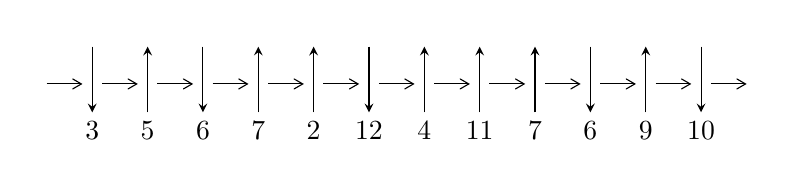
\begin{tikzpicture}[x=20pt, y=17pt]
	% nodes
	\node (C0) at (0, 0) {};
	\node (C1) at (1, 0) {};
	\node (C1U) at (1, +1) {};
	\node (C1D) at (1, -1) {3};

	\node (C2) at (2, 0) {};
	\node (C2U) at (2, +1) {};
	\node (C2D) at (2, -1) {5};

	\node (C3) at (3, 0) {};
	\node (C3U) at (3, +1) {};
	\node (C3D) at (3, -1) {6};

	\node (C4) at (4, 0) {};
	\node (C4U) at (4, +1) {};
	\node (C4D) at (4, -1) {7};

	\node (C5) at (5, 0) {};
	\node (C5U) at (5, +1) {};
	\node (C5D) at (5, -1) {2};

	\node (C6) at (6, 0) {};
	\node (C6U) at (6, +1) {};
	\node (C6D) at (6, -1) {12};

	\node (C7) at (7, 0) {};
	\node (C7U) at (7, +1) {};
	\node (C7D) at (7, -1) {4};

	\node (C8) at (8, 0) {};
	\node (C8U) at (8, +1) {};
	\node (C8D) at (8, -1) {11};

	\node (C9) at (9, 0) {};
	\node (C9U) at (9, +1) {};
	\node (C9D) at (9, -1) {7};

	\node (C10) at (10, 0) {};
	\node (C10U) at (10, +1) {};
	\node (C10D) at (10, -1) {6};

	\node (C11) at (11, 0) {};
	\node (C11U) at (11, +1) {};
	\node (C11D) at (11, -1) {9};

	\node (C12) at (12, 0) {};
	\node (C12U) at (12, +1) {};
	\node (C12D) at (12, -1) {10};
	\node (C13) at (13, 0) {};

	% arrows
	\draw[->,>={angle 60}]
	(C0) edge (C1) (C1) edge (C2) (C2) edge (C3) (C3) edge (C4) (C4) edge (C5) (C5) edge (C6) (C6) edge (C7) (C7) edge (C8) (C8) edge (C9) (C9) edge (C10) (C10) edge (C11) (C11) edge (C12) (C12) edge (C13) ;	\draw[->,>=stealth]
	(C1U) edge (C1D) (C2D) edge (C2U) (C3U) edge (C3D) (C4D) edge (C4U) (C5D) edge (C5U) (C6U) edge (C6D) (C7D) edge (C7U) (C8D) edge (C8U) (C9D) edge (C9U) (C10U) edge (C10D) (C11D) edge (C11U) (C12U) edge (C12D) ;
	\end{tikzpicture} \\
\hhline{~~} \\& 
\textbf{Solving Sequence} \\ \cline{2-2} 
 &
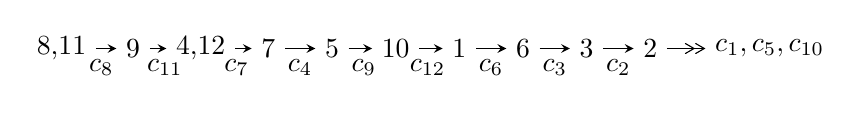
\begin{tikzpicture}[x=23pt, y=7pt]
	% node
	\node (A0) at (-1/8, 0) {8,11};
	\node (A1) at (1, 0) {9};
	\node (A2) at (33/16, 0) {4,12};
	\node (A3) at (25/8, 0) {7};
	\node (A4) at (33/8, 0) {5};
	\node (A5) at (41/8, 0) {10};
	\node (A6) at (49/8, 0) {1};
	\node (A7) at (57/8, 0) {6};
	\node (A8) at (65/8, 0) {3};
	\node (A9) at (73/8, 0) {2};
	\node (C1) at (1/2, -1) {$c_{8}$};
	\node (C2) at (3/2, -1) {$c_{11}$};
	\node (C3) at (21/8, -1) {$c_{7}$};
	\node (C4) at (29/8, -1) {$c_{4}$};
	\node (C5) at (37/8, -1) {$c_{9}$};
	\node (C6) at (45/8, -1) {$c_{12}$};
	\node (C7) at (53/8, -1) {$c_{6}$};
	\node (C8) at (61/8, -1) {$c_{3}$};
	\node (C9) at (69/8, -1) {$c_{2}$};
	\node (A10) at (11, 0) {$c_{1},c_{5},c_{10}$};

	% edge
	\draw[->,>=stealth]	
	(A0) edge (A1) (A1) edge (A2) (A2) edge (A3) (A3) edge (A4) (A4) edge (A5) (A5) edge (A6) (A6) edge (A7) (A7) edge (A8) (A8) edge (A9) ;
	\draw[->>,>={angle 60}]	
	(A9) edge (A10);
\end{tikzpicture} \\ 

\end{tabular} \\

\footnotetext{
The image of knot diagram is generated by the software ``\textbf{Draw programme}" developed by Andrew Bartholomew(\url{http://www.layer8.co.uk/maths/draw/index.htm\#Running-draw}), where we modified some parts for our purpose(\url{https://github.com/CATsTAILs/LinksPainter}).
}\phantom \\ \newline 
\centering \textbf{Ideals for irreducible components\footnotemark of $X_{\text{par}}$} 
 
\begin{align*}
I^u_{1}&=\langle 
3.08304\times10^{52} u^{37}-3.92285\times10^{53} u^{36}+\cdots+2.56521\times10^{53} b-1.92852\times10^{53},\\
\phantom{I^u_{1}}&\phantom{= \langle  }-4.66168\times10^{52} u^{37}+5.98970\times10^{53} u^{36}+\cdots+2.56521\times10^{53} a-4.47281\times10^{53},\\
\phantom{I^u_{1}}&\phantom{= \langle  }u^{38}-13 u^{37}+\cdots-8 u+1\rangle \\
I^u_{2}&=\langle 
b,\;- u^5 a+2 u^4 a+u^5-3 u^4-2 u^2 a+3 u^3+a^2+a u-2 u+1,\;u^6- u^5- u^4+2 u^3- u+1\rangle \\
I^u_{3}&=\langle 
a^3+b+2 a,\;a^4- a^3+3 a^2-2 a+1,\;u+1\rangle \\
I^u_{4}&=\langle 
39 a^5-213 a^4+550 a^3-390 a^2+295 b+748 a-63,\;a^6-5 a^5+11 a^4+7 a^2+2 a+1,\;u+1\rangle \\
\\
\end{align*}
\raggedright * 4 irreducible components of $\dim_{\mathbb{C}}=0$, with total 60 representations.\\
\footnotetext{All coefficients of polynomials are rational numbers. But the coefficients are sometimes approximated in decimal forms when there is not enough margin.}
\newpage
\renewcommand{\arraystretch}{1}
\centering \section*{I. $I^u_{1}= \langle 3.08\times10^{52} u^{37}-3.92\times10^{53} u^{36}+\cdots+2.57\times10^{53} b-1.93\times10^{53},\;-4.66\times10^{52} u^{37}+5.99\times10^{53} u^{36}+\cdots+2.57\times10^{53} a-4.47\times10^{53},\;u^{38}-13 u^{37}+\cdots-8 u+1 \rangle$}
\flushleft \textbf{(i) Arc colorings}\\
\begin{tabular}{m{7pt} m{180pt} m{7pt} m{180pt} }
\flushright $a_{8}=$&$\begin{pmatrix}1\\0\end{pmatrix}$ \\
\flushright $a_{11}=$&$\begin{pmatrix}0\\u\end{pmatrix}$ \\
\flushright $a_{9}=$&$\begin{pmatrix}1\\- u^2\end{pmatrix}$ \\
\flushright $a_{4}=$&$\begin{pmatrix}0.181727 u^{37}-2.33497 u^{36}+\cdots+20.3488 u+1.74364\\-0.120187 u^{37}+1.52925 u^{36}+\cdots-5.67119 u+0.751797\end{pmatrix}$ \\
\flushright $a_{12}=$&$\begin{pmatrix}u\\- u^3+u\end{pmatrix}$ \\
\flushright $a_{7}=$&$\begin{pmatrix}-0.780745 u^{37}+9.98000 u^{36}+\cdots-13.8096 u+4.94182\\0.239039 u^{37}-3.07898 u^{36}+\cdots+2.00450 u-1.30500\end{pmatrix}$ \\
\flushright $a_{5}=$&$\begin{pmatrix}1.05713 u^{37}-13.6449 u^{36}+\cdots+30.2257 u-4.50545\\-0.236519 u^{37}+3.03144 u^{36}+\cdots-6.54670 u+2.04114\end{pmatrix}$ \\
\flushright $a_{10}=$&$\begin{pmatrix}0.187039 u^{37}-2.41394 u^{36}+\cdots-7.46873 u-2.11666\\-0.000250736 u^{37}+0.0152541 u^{36}+\cdots+2.70178 u+0.223799\end{pmatrix}$ \\
\flushright $a_{1}=$&$\begin{pmatrix}0.0174232 u^{37}-0.223414 u^{36}+\cdots+2.06976 u-0.961603\\0.0147652 u^{37}-0.190086 u^{36}+\cdots+2.06249 u+0.0414843\end{pmatrix}$ \\
\flushright $a_{6}=$&$\begin{pmatrix}-0.758911 u^{37}+9.70005 u^{36}+\cdots-13.2564 u+4.74750\\0.261495 u^{37}-3.36527 u^{36}+\cdots+2.54841 u-1.49543\end{pmatrix}$ \\
\flushright $a_{3}=$&$\begin{pmatrix}0.858153 u^{37}-11.0889 u^{36}+\cdots+28.3257 u-4.91506\\-0.174044 u^{37}+2.22800 u^{36}+\cdots-3.74240 u+1.77583\end{pmatrix}$ \\
\flushright $a_{2}=$&$\begin{pmatrix}-0.474366 u^{37}+6.13382 u^{36}+\cdots+28.8620 u+0.288063\\0.0102207 u^{37}-0.155656 u^{36}+\cdots+0.659483 u-0.0673376\end{pmatrix}$\\&\end{tabular}
\flushleft \textbf{(ii) Obstruction class $= -1$}\\~\\
\flushleft \textbf{(iii) Cusp Shapes $= -0.765395 u^{37}+9.83295 u^{36}+\cdots-3.08287 u+7.31166$}\\~\\
\newpage\renewcommand{\arraystretch}{1}
\flushleft \textbf{(iv) u-Polynomials at the component}\newline \\
\begin{tabular}{m{50pt}|m{274pt}}
Crossings & \hspace{64pt}u-Polynomials at each crossing \\
\hline $$\begin{aligned}c_{1}\end{aligned}$$&$\begin{aligned}
&u^{38}+28 u^{37}+\cdots+159 u+1
\end{aligned}$\\
\hline $$\begin{aligned}c_{2},c_{5}\end{aligned}$$&$\begin{aligned}
&u^{38}+8 u^{37}+\cdots+11 u+1
\end{aligned}$\\
\hline $$\begin{aligned}c_{3}\end{aligned}$$&$\begin{aligned}
&u^{38}-8 u^{37}+\cdots+17360 u+1732
\end{aligned}$\\
\hline $$\begin{aligned}c_{4},c_{7}\end{aligned}$$&$\begin{aligned}
&u^{38}+2 u^{37}+\cdots-12288 u+4096
\end{aligned}$\\
\hline $$\begin{aligned}c_{6}\end{aligned}$$&$\begin{aligned}
&u^{38}-4 u^{37}+\cdots-3 u+1
\end{aligned}$\\
\hline $$\begin{aligned}c_{8},c_{11}\end{aligned}$$&$\begin{aligned}
&u^{38}+13 u^{37}+\cdots+8 u+1
\end{aligned}$\\
\hline $$\begin{aligned}c_{9}\end{aligned}$$&$\begin{aligned}
&u^{38}+8 u^{37}+\cdots-149993 u+47809
\end{aligned}$\\
\hline $$\begin{aligned}c_{10}\end{aligned}$$&$\begin{aligned}
&u^{38}+2 u^{37}+\cdots+575973 u+248449
\end{aligned}$\\
\hline $$\begin{aligned}c_{12}\end{aligned}$$&$\begin{aligned}
&u^{38}-3 u^{37}+\cdots-11264 u+1024
\end{aligned}$\\
\hline
\end{tabular}\\~\\
\newpage\renewcommand{\arraystretch}{1}
\flushleft \textbf{(v) Riley Polynomials at the component}\newline \\
\begin{tabular}{m{50pt}|m{274pt}}
Crossings & \hspace{64pt}Riley Polynomials at each crossing \\
\hline $$\begin{aligned}c_{1}\end{aligned}$$&$\begin{aligned}
&y^{38}-28 y^{37}+\cdots-10893 y+1
\end{aligned}$\\
\hline $$\begin{aligned}c_{2},c_{5}\end{aligned}$$&$\begin{aligned}
&y^{38}+28 y^{37}+\cdots+159 y+1
\end{aligned}$\\
\hline $$\begin{aligned}c_{3}\end{aligned}$$&$\begin{aligned}
&y^{38}-84 y^{37}+\cdots+436784552 y+2999824
\end{aligned}$\\
\hline $$\begin{aligned}c_{4},c_{7}\end{aligned}$$&$\begin{aligned}
&y^{38}+70 y^{37}+\cdots+134217728 y+16777216
\end{aligned}$\\
\hline $$\begin{aligned}c_{6}\end{aligned}$$&$\begin{aligned}
&y^{38}+4 y^{37}+\cdots+19 y+1
\end{aligned}$\\
\hline $$\begin{aligned}c_{8},c_{11}\end{aligned}$$&$\begin{aligned}
&y^{38}+y^{37}+\cdots-84 y+1
\end{aligned}$\\
\hline $$\begin{aligned}c_{9}\end{aligned}$$&$\begin{aligned}
&y^{38}+48 y^{37}+\cdots+51838210455 y+2285700481
\end{aligned}$\\
\hline $$\begin{aligned}c_{10}\end{aligned}$$&$\begin{aligned}
&y^{38}-84 y^{37}+\cdots+1086486467931 y+61726905601
\end{aligned}$\\
\hline $$\begin{aligned}c_{12}\end{aligned}$$&$\begin{aligned}
&y^{38}-69 y^{37}+\cdots-7864320 y+1048576
\end{aligned}$\\
\hline
\end{tabular}\\~\\
\newpage\flushleft \textbf{(vi) Complex Volumes and Cusp Shapes}
$$\begin{array}{c|c|c}  
\text{Solutions to }I^u_{1}& \I (\text{vol} + \sqrt{-1}CS) & \text{Cusp shape}\\
 \hline 
\begin{aligned}
u &= \phantom{-}0.872556 + 0.495557 I \\
a &= \phantom{-}0.505994 - 0.202943 I \\
b &= -0.690714 - 0.617908 I\end{aligned}
 & \phantom{-}0.91553 + 4.18220 I & \phantom{-}3.10264 - 7.31279 I \\ \hline\begin{aligned}
u &= \phantom{-}0.872556 - 0.495557 I \\
a &= \phantom{-}0.505994 + 0.202943 I \\
b &= -0.690714 + 0.617908 I\end{aligned}
 & \phantom{-}0.91553 - 4.18220 I & \phantom{-}3.10264 + 7.31279 I \\ \hline\begin{aligned}
u &= -1.029200 + 0.216658 I \\
a &= -0.422423 + 0.457150 I \\
b &= -0.209980 + 0.250980 I\end{aligned}
 & \phantom{-}1.91078 - 0.79833 I & \phantom{-}4.44525 - 0.45789 I \\ \hline\begin{aligned}
u &= -1.029200 - 0.216658 I \\
a &= -0.422423 - 0.457150 I \\
b &= -0.209980 - 0.250980 I\end{aligned}
 & \phantom{-}1.91078 + 0.79833 I & \phantom{-}4.44525 + 0.45789 I \\ \hline\begin{aligned}
u &= -0.933302 + 0.093882 I \\
a &= -2.24303 + 4.72814 I \\
b &= \phantom{-}0.300084 + 0.412662 I\end{aligned}
 & \phantom{-}1.67684 - 2.65330 I & \phantom{-}7.7232 - 16.8130 I \\ \hline\begin{aligned}
u &= -0.933302 - 0.093882 I \\
a &= -2.24303 - 4.72814 I \\
b &= \phantom{-}0.300084 - 0.412662 I\end{aligned}
 & \phantom{-}1.67684 + 2.65330 I & \phantom{-}7.7232 + 16.8130 I \\ \hline\begin{aligned}
u &= -1.130550 + 0.077748 I \\
a &= \phantom{-}1.43764 - 2.54970 I \\
b &= -0.392217 - 0.325280 I\end{aligned}
 & \phantom{-}2.15015 + 1.46241 I & \phantom{-0.000000 } 0. - 14.08993 I \\ \hline\begin{aligned}
u &= -1.130550 - 0.077748 I \\
a &= \phantom{-}1.43764 + 2.54970 I \\
b &= -0.392217 + 0.325280 I\end{aligned}
 & \phantom{-}2.15015 - 1.46241 I & \phantom{-0.000000 -}0. + 14.08993 I \\ \hline\begin{aligned}
u &= \phantom{-}1.094840 + 0.358324 I \\
a &= -0.425261 - 0.241871 I \\
b &= \phantom{-}0.269512 + 0.935520 I\end{aligned}
 & -0.61516 + 8.47206 I & -1.23185 - 12.18265 I \\ \hline\begin{aligned}
u &= \phantom{-}1.094840 - 0.358324 I \\
a &= -0.425261 + 0.241871 I \\
b &= \phantom{-}0.269512 - 0.935520 I\end{aligned}
 & -0.61516 - 8.47206 I & -1.23185 + 12.18265 I\\
 \hline 
 \end{array}$$\newpage$$\begin{array}{c|c|c}  
\text{Solutions to }I^u_{1}& \I (\text{vol} + \sqrt{-1}CS) & \text{Cusp shape}\\
 \hline 
\begin{aligned}
u &= -0.851367 + 0.892503 I \\
a &= -0.001244 - 0.292263 I \\
b &= -0.962152 - 0.487944 I\end{aligned}
 & \phantom{-}0.067821 - 0.704860 I & \phantom{-}2.00000 + 2.96425 I \\ \hline\begin{aligned}
u &= -0.851367 - 0.892503 I \\
a &= -0.001244 + 0.292263 I \\
b &= -0.962152 + 0.487944 I\end{aligned}
 & \phantom{-}0.067821 + 0.704860 I & \phantom{-}2.00000 - 2.96425 I \\ \hline\begin{aligned}
u &= \phantom{-}0.697244 + 0.310286 I \\
a &= \phantom{-}0.159158 + 0.892544 I \\
b &= \phantom{-}0.334991 - 0.821597 I\end{aligned}
 & -3.35491 + 0.78621 I & -8.48784 - 2.29609 I \\ \hline\begin{aligned}
u &= \phantom{-}0.697244 - 0.310286 I \\
a &= \phantom{-}0.159158 - 0.892544 I \\
b &= \phantom{-}0.334991 + 0.821597 I\end{aligned}
 & -3.35491 - 0.78621 I & -8.48784 + 2.29609 I \\ \hline\begin{aligned}
u &= \phantom{-}0.110487 + 0.652381 I \\
a &= -0.913173 + 0.555160 I \\
b &= \phantom{-}0.154768 + 0.641440 I\end{aligned}
 & -1.32113 - 1.32492 I & -1.95750 + 1.98412 I \\ \hline\begin{aligned}
u &= \phantom{-}0.110487 - 0.652381 I \\
a &= -0.913173 - 0.555160 I \\
b &= \phantom{-}0.154768 - 0.641440 I\end{aligned}
 & -1.32113 + 1.32492 I & -1.95750 - 1.98412 I \\ \hline\begin{aligned}
u &= \phantom{-}0.224375 + 1.325980 I \\
a &= \phantom{-}0.096188 + 1.029440 I \\
b &= \phantom{-}1.75400 + 1.85534 I\end{aligned}
 & -6.74677 + 2.59569 I & \phantom{-0.000000 } 0 \\ \hline\begin{aligned}
u &= \phantom{-}0.224375 - 1.325980 I \\
a &= \phantom{-}0.096188 - 1.029440 I \\
b &= \phantom{-}1.75400 - 1.85534 I\end{aligned}
 & -6.74677 - 2.59569 I & \phantom{-0.000000 } 0 \\ \hline\begin{aligned}
u &= -0.281259 + 0.487374 I \\
a &= \phantom{-}1.158940 - 0.418649 I \\
b &= \phantom{-}1.336190 - 0.226899 I\end{aligned}
 & -0.61371 + 2.86891 I & -0.25435 - 4.83204 I \\ \hline\begin{aligned}
u &= -0.281259 - 0.487374 I \\
a &= \phantom{-}1.158940 + 0.418649 I \\
b &= \phantom{-}1.336190 + 0.226899 I\end{aligned}
 & -0.61371 - 2.86891 I & -0.25435 + 4.83204 I\\
 \hline 
 \end{array}$$\newpage$$\begin{array}{c|c|c}  
\text{Solutions to }I^u_{1}& \I (\text{vol} + \sqrt{-1}CS) & \text{Cusp shape}\\
 \hline 
\begin{aligned}
u &= \phantom{-}0.12152 + 1.66606 I \\
a &= \phantom{-}0.019900 - 0.800533 I \\
b &= -1.10703 - 1.69579 I\end{aligned}
 & -6.26733 - 3.08288 I & \phantom{-0.000000 } 0 \\ \hline\begin{aligned}
u &= \phantom{-}0.12152 - 1.66606 I \\
a &= \phantom{-}0.019900 + 0.800533 I \\
b &= -1.10703 + 1.69579 I\end{aligned}
 & -6.26733 + 3.08288 I & \phantom{-0.000000 } 0 \\ \hline\begin{aligned}
u &= \phantom{-}1.40051 + 1.03446 I \\
a &= \phantom{-}1.000780 - 0.696492 I \\
b &= -0.98102 - 2.10542 I\end{aligned}
 & -16.2164 + 7.5794 I & \phantom{-0.000000 } 0 \\ \hline\begin{aligned}
u &= \phantom{-}1.40051 - 1.03446 I \\
a &= \phantom{-}1.000780 + 0.696492 I \\
b &= -0.98102 + 2.10542 I\end{aligned}
 & -16.2164 - 7.5794 I & \phantom{-0.000000 } 0 \\ \hline\begin{aligned}
u &= \phantom{-}1.24001 + 1.25622 I \\
a &= -0.795058 + 0.781650 I \\
b &= \phantom{-}0.41366 + 2.27352 I\end{aligned}
 & -12.39510 + 1.09723 I & \phantom{-0.000000 } 0 \\ \hline\begin{aligned}
u &= \phantom{-}1.24001 - 1.25622 I \\
a &= -0.795058 - 0.781650 I \\
b &= \phantom{-}0.41366 - 2.27352 I\end{aligned}
 & -12.39510 - 1.09723 I & \phantom{-0.000000 } 0 \\ \hline\begin{aligned}
u &= \phantom{-}1.28856 + 1.21540 I \\
a &= \phantom{-}0.770618 - 0.850146 I \\
b &= -0.58138 - 2.41986 I\end{aligned}
 & -12.2225 + 8.2203 I & \phantom{-0.000000 } 0 \\ \hline\begin{aligned}
u &= \phantom{-}1.28856 - 1.21540 I \\
a &= \phantom{-}0.770618 + 0.850146 I \\
b &= -0.58138 + 2.41986 I\end{aligned}
 & -12.2225 - 8.2203 I & \phantom{-0.000000 } 0 \\ \hline\begin{aligned}
u &= \phantom{-}1.45865 + 1.07373 I \\
a &= -0.932042 + 0.820199 I \\
b &= \phantom{-}1.14222 + 2.13195 I\end{aligned}
 & -15.9377 + 14.9717 I & \phantom{-0.000000 } 0 \\ \hline\begin{aligned}
u &= \phantom{-}1.45865 - 1.07373 I \\
a &= -0.932042 - 0.820199 I \\
b &= \phantom{-}1.14222 - 2.13195 I\end{aligned}
 & -15.9377 - 14.9717 I & \phantom{-0.000000 } 0\\
 \hline 
 \end{array}$$\newpage$$\begin{array}{c|c|c}  
\text{Solutions to }I^u_{1}& \I (\text{vol} + \sqrt{-1}CS) & \text{Cusp shape}\\
 \hline 
\begin{aligned}
u &= -0.137741 + 0.126546 I \\
a &= \phantom{-}0.67206 + 4.46519 I \\
b &= \phantom{-}0.730737 + 0.068723 I\end{aligned}
 & -0.42860 - 2.78462 I & \phantom{-}1.78865 + 4.97070 I \\ \hline\begin{aligned}
u &= -0.137741 - 0.126546 I \\
a &= \phantom{-}0.67206 - 4.46519 I \\
b &= \phantom{-}0.730737 - 0.068723 I\end{aligned}
 & -0.42860 + 2.78462 I & \phantom{-}1.78865 - 4.97070 I \\ \hline\begin{aligned}
u &= \phantom{-}0.135837 + 0.044906 I \\
a &= \phantom{-}4.46953 + 0.98915 I \\
b &= -0.615656 - 0.694581 I\end{aligned}
 & \phantom{-}1.12636 + 1.44186 I & \phantom{-}2.40380 - 3.54555 I \\ \hline\begin{aligned}
u &= \phantom{-}0.135837 - 0.044906 I \\
a &= \phantom{-}4.46953 - 0.98915 I \\
b &= -0.615656 + 0.694581 I\end{aligned}
 & \phantom{-}1.12636 - 1.44186 I & \phantom{-}2.40380 + 3.54555 I \\ \hline\begin{aligned}
u &= \phantom{-}1.07616 + 1.52432 I \\
a &= -0.618148 + 0.747510 I \\
b &= -0.22384 + 3.07549 I\end{aligned}
 & -17.7767 + 1.7959 I & \phantom{-0.000000 } 0 \\ \hline\begin{aligned}
u &= \phantom{-}1.07616 - 1.52432 I \\
a &= -0.618148 - 0.747510 I \\
b &= -0.22384 - 3.07549 I\end{aligned}
 & -17.7767 - 1.7959 I & \phantom{-0.000000 } 0 \\ \hline\begin{aligned}
u &= \phantom{-}1.14268 + 1.63665 I \\
a &= \phantom{-}0.559572 - 0.668950 I \\
b &= \phantom{-}0.32782 - 2.75595 I\end{aligned}
 & -17.5824 - 5.0951 I & \phantom{-0.000000 } 0 \\ \hline\begin{aligned}
u &= \phantom{-}1.14268 - 1.63665 I \\
a &= \phantom{-}0.559572 + 0.668950 I \\
b &= \phantom{-}0.32782 + 2.75595 I\end{aligned}
 & -17.5824 + 5.0951 I & \phantom{-0.000000 } 0\\
 \hline 
 \end{array}$$\newpage\newpage\renewcommand{\arraystretch}{1}
\centering \section*{II. $I^u_{2}= \langle b,\;- u^5 a+u^5+\cdots+a^2+1,\;u^6- u^5- u^4+2 u^3- u+1 \rangle$}
\flushleft \textbf{(i) Arc colorings}\\
\begin{tabular}{m{7pt} m{180pt} m{7pt} m{180pt} }
\flushright $a_{8}=$&$\begin{pmatrix}1\\0\end{pmatrix}$ \\
\flushright $a_{11}=$&$\begin{pmatrix}0\\u\end{pmatrix}$ \\
\flushright $a_{9}=$&$\begin{pmatrix}1\\- u^2\end{pmatrix}$ \\
\flushright $a_{4}=$&$\begin{pmatrix}a\\0\end{pmatrix}$ \\
\flushright $a_{12}=$&$\begin{pmatrix}u\\- u^3+u\end{pmatrix}$ \\
\flushright $a_{7}=$&$\begin{pmatrix}1\\0\end{pmatrix}$ \\
\flushright $a_{5}=$&$\begin{pmatrix}a\\0\end{pmatrix}$ \\
\flushright $a_{10}=$&$\begin{pmatrix}- u^2+1\\- u^2\end{pmatrix}$ \\
\flushright $a_{1}=$&$\begin{pmatrix}- u^4+u^2-1\\u^5- u^4-2 u^3+u^2+u-1\end{pmatrix}$ \\
\flushright $a_{6}=$&$\begin{pmatrix}u^4- u^2+1\\- u^5+u^4+2 u^3- u^2- u+1\end{pmatrix}$ \\
\flushright $a_{3}=$&$\begin{pmatrix}a u+2 a\\-2 u^5 a+2 u^3 a-2 u^2 a- a u+2 a\end{pmatrix}$ \\
\flushright $a_{2}=$&$\begin{pmatrix}- u^5+2 u^4+a u-2 u^2+2 a+u\\-2 u^5 a+2 u^3 a-2 u^2 a- a u+2 a\end{pmatrix}$\\&\end{tabular}
\flushleft \textbf{(ii) Obstruction class $= 1$}\\~\\
\flushleft \textbf{(iii) Cusp Shapes $= - u^5 a+5 u^4 a+u^5+u^3 a-7 u^4-5 u^2 a+3 u^3- a u+4 u^2+a-6 u-1$}\\~\\
\newpage\renewcommand{\arraystretch}{1}
\flushleft \textbf{(iv) u-Polynomials at the component}\newline \\
\begin{tabular}{m{50pt}|m{274pt}}
Crossings & \hspace{64pt}u-Polynomials at each crossing \\
\hline $$\begin{aligned}c_{1},c_{3},c_{5}\end{aligned}$$&$\begin{aligned}
&(u^2- u+1)^6
\end{aligned}$\\
\hline $$\begin{aligned}c_{2}\end{aligned}$$&$\begin{aligned}
&(u^2+u+1)^6
\end{aligned}$\\
\hline $$\begin{aligned}c_{4},c_{7}\end{aligned}$$&$\begin{aligned}
&u^{12}
\end{aligned}$\\
\hline $$\begin{aligned}c_{6},c_{9}\end{aligned}$$&$\begin{aligned}
&(u^6-3 u^5+5 u^4-4 u^3+2 u^2- u+1)^2
\end{aligned}$\\
\hline $$\begin{aligned}c_{8},c_{10},c_{12}\end{aligned}$$&$\begin{aligned}
&(u^6- u^5- u^4+2 u^3- u+1)^2
\end{aligned}$\\
\hline $$\begin{aligned}c_{11}\end{aligned}$$&$\begin{aligned}
&(u^6+u^5- u^4-2 u^3+u+1)^2
\end{aligned}$\\
\hline
\end{tabular}\\~\\
\newpage\renewcommand{\arraystretch}{1}
\flushleft \textbf{(v) Riley Polynomials at the component}\newline \\
\begin{tabular}{m{50pt}|m{274pt}}
Crossings & \hspace{64pt}Riley Polynomials at each crossing \\
\hline $$\begin{aligned}c_{1},c_{2},c_{3}\\c_{5}\end{aligned}$$&$\begin{aligned}
&(y^2+y+1)^6
\end{aligned}$\\
\hline $$\begin{aligned}c_{4},c_{7}\end{aligned}$$&$\begin{aligned}
&y^{12}
\end{aligned}$\\
\hline $$\begin{aligned}c_{6},c_{9}\end{aligned}$$&$\begin{aligned}
&(y^6+y^5+5 y^4+6 y^2+3 y+1)^2
\end{aligned}$\\
\hline $$\begin{aligned}c_{8},c_{10},c_{11}\\c_{12}\end{aligned}$$&$\begin{aligned}
&(y^6-3 y^5+5 y^4-4 y^3+2 y^2- y+1)^2
\end{aligned}$\\
\hline
\end{tabular}\\~\\
\newpage\flushleft \textbf{(vi) Complex Volumes and Cusp Shapes}
$$\begin{array}{c|c|c}  
\text{Solutions to }I^u_{2}& \I (\text{vol} + \sqrt{-1}CS) & \text{Cusp shape}\\
 \hline 
\begin{aligned}
u &= -1.002190 + 0.295542 I \\
a &= -0.82520 + 2.42341 I \\
b &= \phantom{-0.000000 } 0\end{aligned}
 & \phantom{-}1.89061 - 2.95419 I & \phantom{-}11.02954 + 8.16480 I \\ \hline\begin{aligned}
u &= -1.002190 + 0.295542 I \\
a &= \phantom{-}2.51133 - 0.49706 I \\
b &= \phantom{-0.000000 } 0\end{aligned}
 & \phantom{-}1.89061 + 1.10558 I & -0.484082 - 0.231437 I \\ \hline\begin{aligned}
u &= -1.002190 - 0.295542 I \\
a &= -0.82520 - 2.42341 I \\
b &= \phantom{-0.000000 } 0\end{aligned}
 & \phantom{-}1.89061 + 2.95419 I & \phantom{-}11.02954 - 8.16480 I \\ \hline\begin{aligned}
u &= -1.002190 - 0.295542 I \\
a &= \phantom{-}2.51133 + 0.49706 I \\
b &= \phantom{-0.000000 } 0\end{aligned}
 & \phantom{-}1.89061 - 1.10558 I & -0.484082 + 0.231437 I \\ \hline\begin{aligned}
u &= \phantom{-}0.428243 + 0.664531 I \\
a &= \phantom{-}0.489858 + 0.681154 I \\
b &= \phantom{-0.000000 } 0\end{aligned}
 & -1.89061 + 1.10558 I & -1.04064 - 1.99047 I \\ \hline\begin{aligned}
u &= \phantom{-}0.428243 + 0.664531 I \\
a &= -0.834826 + 0.083652 I \\
b &= \phantom{-0.000000 } 0\end{aligned}
 & -1.89061 - 2.95419 I & -3.79900 + 4.11613 I \\ \hline\begin{aligned}
u &= \phantom{-}0.428243 - 0.664531 I \\
a &= \phantom{-}0.489858 - 0.681154 I \\
b &= \phantom{-0.000000 } 0\end{aligned}
 & -1.89061 - 1.10558 I & -1.04064 + 1.99047 I \\ \hline\begin{aligned}
u &= \phantom{-}0.428243 - 0.664531 I \\
a &= -0.834826 - 0.083652 I \\
b &= \phantom{-0.000000 } 0\end{aligned}
 & -1.89061 + 2.95419 I & -3.79900 - 4.11613 I \\ \hline\begin{aligned}
u &= \phantom{-}1.073950 + 0.558752 I \\
a &= \phantom{-}0.458424 - 0.081263 I \\
b &= \phantom{-0.000000 } 0\end{aligned}
 & \phantom{-0.000000 -}7.72290 I & \phantom{-}2.83009 - 4.64337 I \\ \hline\begin{aligned}
u &= \phantom{-}1.073950 + 0.558752 I \\
a &= -0.299588 - 0.356375 I \\
b &= \phantom{-0.000000 } 0\end{aligned}
 & \phantom{-0.000000 -}3.66314 I & -2.53591 - 3.55776 I\\
 \hline 
 \end{array}$$\newpage$$\begin{array}{c|c|c}  
\text{Solutions to }I^u_{2}& \I (\text{vol} + \sqrt{-1}CS) & \text{Cusp shape}\\
 \hline 
\begin{aligned}
u &= \phantom{-}1.073950 - 0.558752 I \\
a &= \phantom{-}0.458424 + 0.081263 I \\
b &= \phantom{-0.000000 } 0\end{aligned}
 & \phantom{-0.000000 } -7.72290 I & \phantom{-}2.83009 + 4.64337 I \\ \hline\begin{aligned}
u &= \phantom{-}1.073950 - 0.558752 I \\
a &= -0.299588 + 0.356375 I \\
b &= \phantom{-0.000000 } 0\end{aligned}
 & \phantom{-0.000000 } -3.66314 I & -2.53591 + 3.55776 I\\
 \hline 
 \end{array}$$\newpage\newpage\renewcommand{\arraystretch}{1}
\centering \section*{III. $I^u_{3}= \langle a^3+b+2 a,\;a^4- a^3+3 a^2-2 a+1,\;u+1 \rangle$}
\flushleft \textbf{(i) Arc colorings}\\
\begin{tabular}{m{7pt} m{180pt} m{7pt} m{180pt} }
\flushright $a_{8}=$&$\begin{pmatrix}1\\0\end{pmatrix}$ \\
\flushright $a_{11}=$&$\begin{pmatrix}0\\-1\end{pmatrix}$ \\
\flushright $a_{9}=$&$\begin{pmatrix}1\\-1\end{pmatrix}$ \\
\flushright $a_{4}=$&$\begin{pmatrix}a\\- a^3-2 a\end{pmatrix}$ \\
\flushright $a_{12}=$&$\begin{pmatrix}-1\\0\end{pmatrix}$ \\
\flushright $a_{7}=$&$\begin{pmatrix}- a^3+a^2-2 a+2\\a^3- a^2+3 a-2\end{pmatrix}$ \\
\flushright $a_{5}=$&$\begin{pmatrix}- a^3- a-1\\- a^3+a^2-2 a+2\end{pmatrix}$ \\
\flushright $a_{10}=$&$\begin{pmatrix}- a^2\\0\end{pmatrix}$ \\
\flushright $a_{1}=$&$\begin{pmatrix}-1\\0\end{pmatrix}$ \\
\flushright $a_{6}=$&$\begin{pmatrix}a\\a^3- a^2+3 a-2\end{pmatrix}$ \\
\flushright $a_{3}=$&$\begin{pmatrix}a^2+a+1\\a^3- a^2+3 a-2\end{pmatrix}$ \\
\flushright $a_{2}=$&$\begin{pmatrix}- a^3+a^2-2 a+2\\2 a^3- a^2+5 a-1\end{pmatrix}$\\&\end{tabular}
\flushleft \textbf{(ii) Obstruction class $= 1$}\\~\\
\flushleft \textbf{(iii) Cusp Shapes $= -7 a^2-2 a-3$}\\~\\
\newpage\renewcommand{\arraystretch}{1}
\flushleft \textbf{(iv) u-Polynomials at the component}\newline \\
\begin{tabular}{m{50pt}|m{274pt}}
Crossings & \hspace{64pt}u-Polynomials at each crossing \\
\hline $$\begin{aligned}c_{1}\end{aligned}$$&$\begin{aligned}
&u^4-2 u^3+3 u^2- u+1
\end{aligned}$\\
\hline $$\begin{aligned}c_{2},c_{4}\end{aligned}$$&$\begin{aligned}
&u^4+u^2+u+1
\end{aligned}$\\
\hline $$\begin{aligned}c_{3}\end{aligned}$$&$\begin{aligned}
&u^4+3 u^3+4 u^2+3 u+2
\end{aligned}$\\
\hline $$\begin{aligned}c_{5},c_{7}\end{aligned}$$&$\begin{aligned}
&u^4+u^2- u+1
\end{aligned}$\\
\hline $$\begin{aligned}c_{6}\end{aligned}$$&$\begin{aligned}
&u^4+2 u^3+3 u^2+u+1
\end{aligned}$\\
\hline $$\begin{aligned}c_{8}\end{aligned}$$&$\begin{aligned}
&(u+1)^4
\end{aligned}$\\
\hline $$\begin{aligned}c_{9},c_{10}\end{aligned}$$&$\begin{aligned}
&u^4- u^3+3 u^2-2 u+1
\end{aligned}$\\
\hline $$\begin{aligned}c_{11}\end{aligned}$$&$\begin{aligned}
&(u-1)^4
\end{aligned}$\\
\hline $$\begin{aligned}c_{12}\end{aligned}$$&$\begin{aligned}
&u^4
\end{aligned}$\\
\hline
\end{tabular}\\~\\
\newpage\renewcommand{\arraystretch}{1}
\flushleft \textbf{(v) Riley Polynomials at the component}\newline \\
\begin{tabular}{m{50pt}|m{274pt}}
Crossings & \hspace{64pt}Riley Polynomials at each crossing \\
\hline $$\begin{aligned}c_{1},c_{6}\end{aligned}$$&$\begin{aligned}
&y^4+2 y^3+7 y^2+5 y+1
\end{aligned}$\\
\hline $$\begin{aligned}c_{2},c_{4},c_{5}\\c_{7}\end{aligned}$$&$\begin{aligned}
&y^4+2 y^3+3 y^2+y+1
\end{aligned}$\\
\hline $$\begin{aligned}c_{3}\end{aligned}$$&$\begin{aligned}
&y^4- y^3+2 y^2+7 y+4
\end{aligned}$\\
\hline $$\begin{aligned}c_{8},c_{11}\end{aligned}$$&$\begin{aligned}
&(y-1)^4
\end{aligned}$\\
\hline $$\begin{aligned}c_{9},c_{10}\end{aligned}$$&$\begin{aligned}
&y^4+5 y^3+7 y^2+2 y+1
\end{aligned}$\\
\hline $$\begin{aligned}c_{12}\end{aligned}$$&$\begin{aligned}
&y^4
\end{aligned}$\\
\hline
\end{tabular}\\~\\
\newpage\flushleft \textbf{(vi) Complex Volumes and Cusp Shapes}
$$\begin{array}{c|c|c}  
\text{Solutions to }I^u_{3}& \I (\text{vol} + \sqrt{-1}CS) & \text{Cusp shape}\\
 \hline 
\begin{aligned}
u &= -1.00000\phantom{ +0.000000I} \\
a &= \phantom{-}0.395123 + 0.506844 I \\
b &= -0.547424 - 1.120870 I\end{aligned}
 & -0.98010 + 7.64338 I & -3.08487 - 3.81741 I \\ \hline\begin{aligned}
u &= -1.00000\phantom{ +0.000000I} \\
a &= \phantom{-}0.395123 - 0.506844 I \\
b &= -0.547424 + 1.120870 I\end{aligned}
 & -0.98010 - 7.64338 I & -3.08487 + 3.81741 I \\ \hline\begin{aligned}
u &= -1.00000\phantom{ +0.000000I} \\
a &= \phantom{-}0.10488 + 1.55249 I \\
b &= \phantom{-}0.547424 + 0.585652 I\end{aligned}
 & \phantom{-}2.62503 + 1.39709 I & \phantom{-}13.5849 - 5.3845 I \\ \hline\begin{aligned}
u &= -1.00000\phantom{ +0.000000I} \\
a &= \phantom{-}0.10488 - 1.55249 I \\
b &= \phantom{-}0.547424 - 0.585652 I\end{aligned}
 & \phantom{-}2.62503 - 1.39709 I & \phantom{-}13.5849 + 5.3845 I\\
 \hline 
 \end{array}$$\newpage\newpage\renewcommand{\arraystretch}{1}
\centering \section*{IV. $I^u_{4}= \langle 39 a^5+295 b+\cdots+748 a-63,\;a^6-5 a^5+11 a^4+7 a^2+2 a+1,\;u+1 \rangle$}
\flushleft \textbf{(i) Arc colorings}\\
\begin{tabular}{m{7pt} m{180pt} m{7pt} m{180pt} }
\flushright $a_{8}=$&$\begin{pmatrix}1\\0\end{pmatrix}$ \\
\flushright $a_{11}=$&$\begin{pmatrix}0\\-1\end{pmatrix}$ \\
\flushright $a_{9}=$&$\begin{pmatrix}1\\-1\end{pmatrix}$ \\
\flushright $a_{4}=$&$\begin{pmatrix}a\\-0.132203 a^{5}+0.722034 a^{4}+\cdots-2.53559 a+0.213559\end{pmatrix}$ \\
\flushright $a_{12}=$&$\begin{pmatrix}-1\\0\end{pmatrix}$ \\
\flushright $a_{7}=$&$\begin{pmatrix}0.0610169 a^{5}-0.410169 a^{4}+\cdots+0.477966 a+1.13220\\-0.369492 a^{5}+2.09492 a^{4}+\cdots-2.06102 a-0.633898\end{pmatrix}$ \\
\flushright $a_{5}=$&$\begin{pmatrix}0.115254 a^{5}-0.552542 a^{4}+\cdots-1.43051 a+0.583051\\-0.593220 a^{5}+2.93220 a^{4}+\cdots-2.81356 a-1.11864\end{pmatrix}$ \\
\flushright $a_{10}=$&$\begin{pmatrix}0.379661 a^{5}-1.99661 a^{4}+\cdots+1.64068 a+0.155932\\0\end{pmatrix}$ \\
\flushright $a_{1}=$&$\begin{pmatrix}-1\\0\end{pmatrix}$ \\
\flushright $a_{6}=$&$\begin{pmatrix}-0.308475 a^{5}+1.68475 a^{4}+\cdots-1.58305 a+0.498305\\-0.369492 a^{5}+2.09492 a^{4}+\cdots-2.06102 a-0.633898\end{pmatrix}$ \\
\flushright $a_{3}=$&$\begin{pmatrix}-0.213559 a^{5}+0.935593 a^{4}+\cdots+0.827119 a-0.962712\\0.522034 a^{5}-2.62034 a^{4}+\cdots+1.75593 a+0.464407\end{pmatrix}$ \\
\flushright $a_{2}=$&$\begin{pmatrix}0.0813559 a^{5}-0.213559 a^{4}+\cdots+1.63729 a+0.176271\\0.176271 a^{5}-0.962712 a^{4}+\cdots-0.952542 a-0.284746\end{pmatrix}$\\&\end{tabular}
\flushleft \textbf{(ii) Obstruction class $= 1$}\\~\\
\flushleft \textbf{(iii) Cusp Shapes $= \frac{119}{59} a^5-\frac{600}{59} a^4+\frac{1300}{59} a^3+\frac{108}{59} a^2+\frac{411}{59} a+\frac{189}{59}$}\\~\\
\newpage\renewcommand{\arraystretch}{1}
\flushleft \textbf{(iv) u-Polynomials at the component}\newline \\
\begin{tabular}{m{50pt}|m{274pt}}
Crossings & \hspace{64pt}u-Polynomials at each crossing \\
\hline $$\begin{aligned}c_{1}\end{aligned}$$&$\begin{aligned}
&u^6-3 u^5+4 u^4-2 u^3+1
\end{aligned}$\\
\hline $$\begin{aligned}c_{2},c_{4}\end{aligned}$$&$\begin{aligned}
&u^6- u^5+2 u^4-2 u^3+2 u^2-2 u+1
\end{aligned}$\\
\hline $$\begin{aligned}c_{3}\end{aligned}$$&$\begin{aligned}
&(u^3- u^2+1)^2
\end{aligned}$\\
\hline $$\begin{aligned}c_{5},c_{7}\end{aligned}$$&$\begin{aligned}
&u^6+u^5+2 u^4+2 u^3+2 u^2+2 u+1
\end{aligned}$\\
\hline $$\begin{aligned}c_{6}\end{aligned}$$&$\begin{aligned}
&u^6+3 u^5+4 u^4+2 u^3+1
\end{aligned}$\\
\hline $$\begin{aligned}c_{8}\end{aligned}$$&$\begin{aligned}
&(u+1)^6
\end{aligned}$\\
\hline $$\begin{aligned}c_{9},c_{10}\end{aligned}$$&$\begin{aligned}
&u^6-2 u^3+4 u^2-3 u+1
\end{aligned}$\\
\hline $$\begin{aligned}c_{11}\end{aligned}$$&$\begin{aligned}
&(u-1)^6
\end{aligned}$\\
\hline $$\begin{aligned}c_{12}\end{aligned}$$&$\begin{aligned}
&u^6
\end{aligned}$\\
\hline
\end{tabular}\\~\\
\newpage\renewcommand{\arraystretch}{1}
\flushleft \textbf{(v) Riley Polynomials at the component}\newline \\
\begin{tabular}{m{50pt}|m{274pt}}
Crossings & \hspace{64pt}Riley Polynomials at each crossing \\
\hline $$\begin{aligned}c_{1},c_{6}\end{aligned}$$&$\begin{aligned}
&y^6- y^5+4 y^4-2 y^3+8 y^2+1
\end{aligned}$\\
\hline $$\begin{aligned}c_{2},c_{4},c_{5}\\c_{7}\end{aligned}$$&$\begin{aligned}
&y^6+3 y^5+4 y^4+2 y^3+1
\end{aligned}$\\
\hline $$\begin{aligned}c_{3}\end{aligned}$$&$\begin{aligned}
&(y^3- y^2+2 y-1)^2
\end{aligned}$\\
\hline $$\begin{aligned}c_{8},c_{11}\end{aligned}$$&$\begin{aligned}
&(y-1)^6
\end{aligned}$\\
\hline $$\begin{aligned}c_{9},c_{10}\end{aligned}$$&$\begin{aligned}
&y^6+8 y^4-2 y^3+4 y^2- y+1
\end{aligned}$\\
\hline $$\begin{aligned}c_{12}\end{aligned}$$&$\begin{aligned}
&y^6
\end{aligned}$\\
\hline
\end{tabular}\\~\\
\newpage\flushleft \textbf{(vi) Complex Volumes and Cusp Shapes}
$$\begin{array}{c|c|c}  
\text{Solutions to }I^u_{4}& \I (\text{vol} + \sqrt{-1}CS) & \text{Cusp shape}\\
 \hline 
\begin{aligned}
u &= -1.00000\phantom{ +0.000000I} \\
a &= \phantom{-}0.052721 + 0.753034 I \\
b &= -0.284920 - 1.115140 I\end{aligned}
 & -2.75839\phantom{ +0.000000I} & -2.43992 - 2.50363 I \\ \hline\begin{aligned}
u &= -1.00000\phantom{ +0.000000I} \\
a &= \phantom{-}0.052721 - 0.753034 I \\
b &= -0.284920 + 1.115140 I\end{aligned}
 & -2.75839\phantom{ +0.000000I} & -2.43992 + 2.50363 I \\ \hline\begin{aligned}
u &= -1.00000\phantom{ +0.000000I} \\
a &= -0.195217 + 0.332027 I \\
b &= \phantom{-}0.498832 - 1.001300 I\end{aligned}
 & \phantom{-}1.37919 - 2.82812 I & \phantom{-}3.08014 + 1.90022 I \\ \hline\begin{aligned}
u &= -1.00000\phantom{ +0.000000I} \\
a &= -0.195217 - 0.332027 I \\
b &= \phantom{-}0.498832 + 1.001300 I\end{aligned}
 & \phantom{-}1.37919 + 2.82812 I & \phantom{-}3.08014 - 1.90022 I \\ \hline\begin{aligned}
u &= -1.00000\phantom{ +0.000000I} \\
a &= \phantom{-}2.64250 + 2.20145 I \\
b &= -0.713912 + 0.305839 I\end{aligned}
 & \phantom{-}1.37919 + 2.82812 I & -2.14022 - 3.69351 I \\ \hline\begin{aligned}
u &= -1.00000\phantom{ +0.000000I} \\
a &= \phantom{-}2.64250 - 2.20145 I \\
b &= -0.713912 - 0.305839 I\end{aligned}
 & \phantom{-}1.37919 - 2.82812 I & -2.14022 + 3.69351 I\\
 \hline 
 \end{array}$$\newpage
\newpage\renewcommand{\arraystretch}{1}
\centering \section*{ V. u-Polynomials}
\begin{tabular}{m{50pt}|m{274pt}}
Crossings & \hspace{64pt}u-Polynomials at each crossing \\
\hline $$\begin{aligned}c_{1}\end{aligned}$$&$\begin{aligned}
&(u^2- u+1)^6(u^4-2 u^3+3 u^2- u+1)(u^6-3 u^5+4 u^4-2 u^3+1)\\
&\cdot(u^{38}+28 u^{37}+\cdots+159 u+1)
\end{aligned}$\\
\hline $$\begin{aligned}c_{2}\end{aligned}$$&$\begin{aligned}
&(u^2+u+1)^6(u^4+u^2+u+1)(u^6- u^5+2 u^4-2 u^3+2 u^2-2 u+1)\\
&\cdot(u^{38}+8 u^{37}+\cdots+11 u+1)
\end{aligned}$\\
\hline $$\begin{aligned}c_{3}\end{aligned}$$&$\begin{aligned}
&(u^2- u+1)^6(u^3- u^2+1)^2(u^4+3 u^3+4 u^2+3 u+2)\\
&\cdot(u^{38}-8 u^{37}+\cdots+17360 u+1732)
\end{aligned}$\\
\hline $$\begin{aligned}c_{4}\end{aligned}$$&$\begin{aligned}
&u^{12}(u^4+u^2+u+1)(u^6- u^5+2 u^4-2 u^3+2 u^2-2 u+1)\\
&\cdot(u^{38}+2 u^{37}+\cdots-12288 u+4096)
\end{aligned}$\\
\hline $$\begin{aligned}c_{5}\end{aligned}$$&$\begin{aligned}
&(u^2- u+1)^6(u^4+u^2- u+1)(u^6+u^5+2 u^4+2 u^3+2 u^2+2 u+1)\\
&\cdot(u^{38}+8 u^{37}+\cdots+11 u+1)
\end{aligned}$\\
\hline $$\begin{aligned}c_{6}\end{aligned}$$&$\begin{aligned}
&(u^4+2 u^3+3 u^2+u+1)(u^6-3 u^5+5 u^4-4 u^3+2 u^2- u+1)^2\\
&\cdot(u^6+3 u^5+4 u^4+2 u^3+1)(u^{38}-4 u^{37}+\cdots-3 u+1)
\end{aligned}$\\
\hline $$\begin{aligned}c_{7}\end{aligned}$$&$\begin{aligned}
&u^{12}(u^4+u^2- u+1)(u^6+u^5+2 u^4+2 u^3+2 u^2+2 u+1)\\
&\cdot(u^{38}+2 u^{37}+\cdots-12288 u+4096)
\end{aligned}$\\
\hline $$\begin{aligned}c_{8}\end{aligned}$$&$\begin{aligned}
&((u+1)^{10})(u^6- u^5+\cdots- u+1)^{2}(u^{38}+13 u^{37}+\cdots+8 u+1)
\end{aligned}$\\
\hline $$\begin{aligned}c_{9}\end{aligned}$$&$\begin{aligned}
&(u^4- u^3+3 u^2-2 u+1)(u^6-2 u^3+4 u^2-3 u+1)\\
&\cdot(u^6-3 u^5+5 u^4-4 u^3+2 u^2- u+1)^2\\
&\cdot(u^{38}+8 u^{37}+\cdots-149993 u+47809)
\end{aligned}$\\
\hline $$\begin{aligned}c_{10}\end{aligned}$$&$\begin{aligned}
&(u^4- u^3+3 u^2-2 u+1)(u^6-2 u^3+4 u^2-3 u+1)\\
&\cdot((u^6- u^5- u^4+2 u^3- u+1)^2)(u^{38}+2 u^{37}+\cdots+575973 u+248449)
\end{aligned}$\\
\hline $$\begin{aligned}c_{11}\end{aligned}$$&$\begin{aligned}
&((u-1)^{10})(u^6+u^5+\cdots+u+1)^{2}(u^{38}+13 u^{37}+\cdots+8 u+1)
\end{aligned}$\\
\hline $$\begin{aligned}c_{12}\end{aligned}$$&$\begin{aligned}
&u^{10}(u^6- u^5+\cdots- u+1)^{2}(u^{38}-3 u^{37}+\cdots-11264 u+1024)
\end{aligned}$\\
\hline
\end{tabular}\newpage\renewcommand{\arraystretch}{1}
\centering \section*{ VI. Riley Polynomials}
\begin{tabular}{m{50pt}|m{274pt}}
Crossings & \hspace{64pt}Riley Polynomials at each crossing \\
\hline $$\begin{aligned}c_{1}\end{aligned}$$&$\begin{aligned}
&((y^2+y+1)^6)(y^4+2 y^3+\cdots+5 y+1)(y^6- y^5+\cdots+8 y^2+1)\\
&\cdot(y^{38}-28 y^{37}+\cdots-10893 y+1)
\end{aligned}$\\
\hline $$\begin{aligned}c_{2},c_{5}\end{aligned}$$&$\begin{aligned}
&(y^2+y+1)^6(y^4+2 y^3+3 y^2+y+1)(y^6+3 y^5+4 y^4+2 y^3+1)\\
&\cdot(y^{38}+28 y^{37}+\cdots+159 y+1)
\end{aligned}$\\
\hline $$\begin{aligned}c_{3}\end{aligned}$$&$\begin{aligned}
&(y^2+y+1)^6(y^3- y^2+2 y-1)^2(y^4- y^3+2 y^2+7 y+4)\\
&\cdot(y^{38}-84 y^{37}+\cdots+436784552 y+2999824)
\end{aligned}$\\
\hline $$\begin{aligned}c_{4},c_{7}\end{aligned}$$&$\begin{aligned}
&y^{12}(y^4+2 y^3+3 y^2+y+1)(y^6+3 y^5+4 y^4+2 y^3+1)\\
&\cdot(y^{38}+70 y^{37}+\cdots+134217728 y+16777216)
\end{aligned}$\\
\hline $$\begin{aligned}c_{6}\end{aligned}$$&$\begin{aligned}
&(y^4+2 y^3+7 y^2+5 y+1)(y^6- y^5+4 y^4-2 y^3+8 y^2+1)\\
&\cdot((y^6+y^5+5 y^4+6 y^2+3 y+1)^2)(y^{38}+4 y^{37}+\cdots+19 y+1)
\end{aligned}$\\
\hline $$\begin{aligned}c_{8},c_{11}\end{aligned}$$&$\begin{aligned}
&(y-1)^{10}(y^6-3 y^5+5 y^4-4 y^3+2 y^2- y+1)^2\\
&\cdot(y^{38}+y^{37}+\cdots-84 y+1)
\end{aligned}$\\
\hline $$\begin{aligned}c_{9}\end{aligned}$$&$\begin{aligned}
&(y^4+5 y^3+7 y^2+2 y+1)(y^6+8 y^4-2 y^3+4 y^2- y+1)\\
&\cdot(y^6+y^5+5 y^4+6 y^2+3 y+1)^2\\
&\cdot(y^{38}+48 y^{37}+\cdots+51838210455 y+2285700481)
\end{aligned}$\\
\hline $$\begin{aligned}c_{10}\end{aligned}$$&$\begin{aligned}
&(y^4+5 y^3+7 y^2+2 y+1)(y^6+8 y^4-2 y^3+4 y^2- y+1)\\
&\cdot(y^6-3 y^5+5 y^4-4 y^3+2 y^2- y+1)^2\\
&\cdot(y^{38}-84 y^{37}+\cdots+1086486467931 y+61726905601)
\end{aligned}$\\
\hline $$\begin{aligned}c_{12}\end{aligned}$$&$\begin{aligned}
&y^{10}(y^6-3 y^5+5 y^4-4 y^3+2 y^2- y+1)^2\\
&\cdot(y^{38}-69 y^{37}+\cdots-7864320 y+1048576)
\end{aligned}$\\
\hline
\end{tabular}
\vskip 2pc
\end{document}